%%******************************************************************************
%%
%% body05.tex
%%
%%******************************************************************************
%%
%% Title......: DORIS - Offshore Facilities Monitoring Robots
%%
%% Author.....: COPPE/LEAD-UFRJ Team - G2 (Embedded Electronics)
%%
%% Started....:      Fri Feb 01 2013
%% Last Modified...: Fri Jun 10 2013
%%
%% Emails.....: liu@coep.ufrj.br
%%              jacoud@poli.ufrj.br
%%              marco.fsantosx@gmail.com
%%              renan028@gmail.com
%%
%% Address....: Universidade Federal do Rio de Janeiro
%%              Caixa Postal 68.504, CEP: 21.945-970
%%              Rio de Janeiro, RJ - Brasil.
%%
%%******************************************************************************


%%******************************************************************************
%% CHAPTER - Proposed Spatial Layouts
%%******************************************************************************


\chapter{Wiring and Connections} \label{CHAPTER_WIRING}
This chapter presents in detail the methodology for specification of cables and connectors used in electronics architecture, such as:
\begin{itemize}
    \item Communication cables:
    \begin{itemize}
        \item Ethernet/LAN;
        \item Controller Area Network (CAN);
        \item Universal Serial Bus (USB).
    \end{itemize}
    \item Electrical cables:
    \begin{itemize}
        \item For instruments (e.g.: 4-20 mA, voltage, etc.);
        \item For connection over/between printed circuit boards.
    \end{itemize}
\end{itemize}
Specification of cables for power supply system are under G3 (Power Supply Group) scope.
\newpage


%%******************************************************************************
%% SECTION - Section
%%******************************************************************************


\section{Tagging} \label{CABLE_TAGGING}
In order to organize the list of necessary cables for electronics, we shall propose a technical tagging system to use as a standard in this report (figure~\ref{FIG:TAGGING}):


\begin{figure}[H]
  \centering
  % Requires \usepackage{graphicx}
  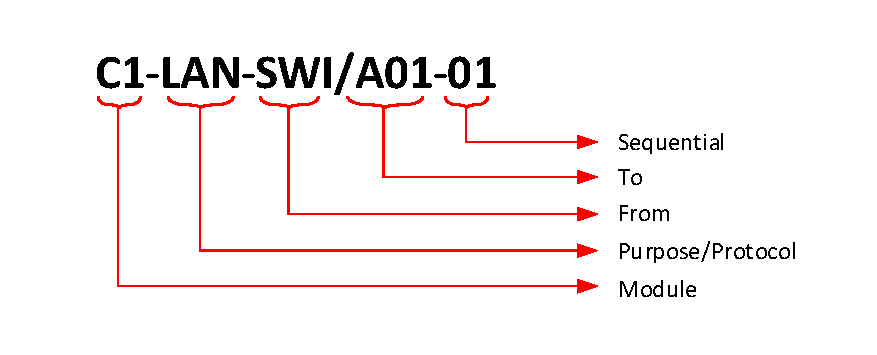
\includegraphics[width=1\columnwidth]{figs/tables/Tagging.pdf}\\
  \caption[Cable tagging standard]{Cable tagging standard.}
  \label{FIG:TAGGING}
\end{figure}

\begin{itemize}
    \item \textbf{Module}: "C" denotes "cable". The second digit is the identifier of the module in which the cable is installed (in the example, module 1). For cables linking two modules, we shall use "CM".
    \item \textbf{Purpose/Protocol}: Three characters code for the type of signal/protocol or purpose of the cable (e.g.: LAN (Local Area Network - Ethernet), CAN (Controller Area Network), USB (Universal Serial Bus), ANA (Analog), etc.);
    \item \textbf{From/To}: Origin (maximum of four characters)/Destination (maximum of four characters) of the cable, always taking direction towards the network "interior", e.g.: Module 2 cable inlet/outlet to switch, switch to PC, PC to camera, PC to sensor, etc. We shall use the following acronyms:
        \begin{itemize}
            \item FORE - Cable inlet/outlet of one module's side (chosen as "front side");
            \item REAR - Cable inlet/outlet of one module's side (chosen as "rear side");
            \item SWI - Ethernet switch;
            \item PC - Computer/PC;
            \item CAN - LAN/CAN Gateway;
            \item I2C - LAN/I2C Gateway;
            \item AP - Access Point;
            \item CA* - CA1 (Camera 1), CA2 (Camera 2), etc.;
            \item AU* - AU1 (Audio 1), AU2 (Audio 2), etc.;
            \item DR* - DR1 (Motor 1 Driver), DR2 (Motor 2 Driver), etc.;
            \item MT* - MT1 (Motor 1), MT2 (Motor 2), etc.;
            \item DAQ - Data acquisition board;
            \item S** - S01 (Sensor 01), S02 (Sensor 02), etc.;
            \item D** - General devices (e.g.: D01 - General device 01, etc.);
            \item M* - For cables linking two modules, we shall use, for example, "M1/M2", always taking the lower index before (M1).
        \end{itemize}
    \item \textbf{Sequential}: two digit sequential to distinguish cables linking the same origin and destinations.
\end{itemize}

For example, a cable tagged as "C3-LAN-SWI/CAN-01" would be a ethernet cable to be installed within module no. 3 to connect its ethernet switch to the LAN/CAN gateway.

\section{Cable Summary List} \label{CABLE_LIST}
At this moment, we surve